\documentclass{article}
\usepackage[T1]{fontenc}
\usepackage{textcomp}
\usepackage{listings}
\usepackage[shortlabels]{enumitem}
\usepackage{caption}
\usepackage{subcaption}
\usepackage{amsmath}
\usepackage{amssymb}
\usepackage{mathtools}
\usepackage[margin=0.75in]{geometry}
\usepackage{fancyhdr}
\usepackage{xcolor}
\usepackage{tikz}
\usetikzlibrary{backgrounds}
\usetikzlibrary{calc}
\usepackage[normalem]{ulem} % for strike through text
\setlength{\headheight}{0in} 
\newcommand{\problemsep}{\leavevmode\\[0.05in] \rule[\baselineskip/4]{\textwidth}{1pt} \\[0.005in] \rule[\baselineskip]{\textwidth}{1pt}\vspace{-\baselineskip}\leavevmode\\[0.05in]}
\newcommand{\statementsep}{\leavevmode\\[0.005in] \rule[\baselineskip/4]{\textwidth}{0.4pt}\leavevmode\\[0.005in]}
\pagestyle{fancy}
\rhead{\today}
\lhead{Daniel Mortensen}
\chead{Programming Assignment 1}
\definecolor{commentsColor}{rgb}{0.497495, 0.497587, 0.497464}
\definecolor{keywordsColor}{rgb}{0.000000, 0.000000, 0.635294}
\definecolor{stringColor}{rgb}{0.558215, 0.000000, 0.135316}
\lstset{%
title=\lstname,
upquote=true,
showstringspaces=false,
breaklines=true,
basicstyle=\footnotesize,
commentstyle=\color{commentsColor}\textit,
keywordstyle=\color{keywordsColor}\bfseries,
numberstyle=\tiny\color{commentsColor},
language=c++,
numbers=left,
stringstyle=\color{stringColor},
rulecolor=\color{black},
frame=tb,
tabsize=4,
columns=fixed,
captionpos=t,
}
\begin{document}
% problem 1
\noindent\underline{Preliminary Exercises}: Show that if $X$ is a random variable with mean $0$ and variance $1$ then
\begin{equation*}
	Y = aX + b 
\end{equation*}
is a random variable with mean $b$ and variance $a^2$.
\statementsep
{\it Claim: } $E[X] = 0$, $E[X^2] = 1$, and $Y = aX + b \implies E[Y] = a$ \\[0.05in]
{\it Proof: } First, we compute the mean. Recall that the mean of a random variable $Y$is defined as the expected value of $Y$ so that
\begin{equation*}\begin{aligned}
	E[Y] &= E[aX + b] \\
       &= aE[X] + b \\
\end{aligned}\end{equation*}
but because $X$ is zero-mean, then $E[X] = 0$ so that
\begin{equation*}
	E[Y] = aE[X] + b\\ \implies E[Y] = b.
\end{equation*}
Therefore, the mean of $Y$ is equal to $b$.\\[0.2in]
{\it Claim: } $Y = aX + b$, $E[X] = 0$, and $E[X^2] = 1$ $\implies \text{Var}(Y) = a^2$ \\[0.05in]
{\it Proof: } Next, we show that the variance is equal to $a^2$. Begin by recalling that the variance is the expected squared difference from the mean, or that
\begin{equation*}
	\text{Var}(Y) = E[(Y - b)^2]
\end{equation*}
as the mean is equal to $b$ per our last proof. Therefore, 
\begin{equation*}\begin{aligned}
	\text{Var}(Y) = E[(Y - b)^2] &\implies \text{Var}(Y) = E[Y^2] - 2bE[Y] + b^2 \\
                           		 &\implies \text{Var}(Y) = E[(aX + b)^2] - 2bE[aX + b] + b^2\\
								               &\implies \text{Var}(Y) = \left [ E[a^2X^2] + 2E[abX] + b^2 \right ] - \left [ 2abE[X] + 2b^2 \right ] + b^2 \\
															 &\implies \text{Var}(Y) = a^2E[X^2] + 2abE[X] - 2abE[X]\\
															 &\implies \text{Var}(Y) = a^2E[X^2] \\
													     &\implies \text{Var}(Y) = a^2
\end{aligned}\end{equation*} 
\problemsep 
\pagebreak \begin{center} \vspace{-0.2in} \underline{BPSK Simulation} \end{center}
\begin{enumerate}
	\item {\it Prompt: } Write a program that will simulate a BPSK communication system with unequal prior bit probabilities. Using your program, create data from which to plot the probability of bit error obtained from your simulation for SNRs in the range from 0 to 10 dB, for the three cases that $P_0 = 0.5$ (in which case your plot should look much like Figure 1.10), $p_0 = 0.25$, and $P_0 = 0.1$. Decide on an appropriate value of $N$\\[0.05in]
				{\it Response: } We accomplish this objective by constructing a {\it Source}, {\it Constellation}, and {\it ConstellationChannel} class.  The source class is responsible for producing input bits which are equal to $1$ with probability $P_0$. The constellation class is responsible for encoding bits to and decoding bits from a constellation of $n$ symbols. Finally, the constellationChannel class adds uncorrelated white gaussian noise with variance $\sigma^2$ to an input set of symbols that come from encoding using the Constellation class.
\lstinputlisting{src/Source.h}
\lstinputlisting{src/Constellation.h}
\lstinputlisting{src/ConstellationChannel.h}
Error metrics are computed using a {\it PerformanceMetrics} class which computs both theoretical and actual error metrics.
\lstinputlisting{src/PerformanceMetric.h}
Each class is used together as follows:
\lstinputlisting{src/main.cpp}
\item {\it Prompt: } Prepare data from which to plot the theoretical probability of error (1.24) for the same three values of $P_0$. (You may want to combinen these first two programs into a single program). \\[0.05in]
			{\it Response: } This was accomplished by implementing equation 1.24 as part of the PerformanceMetric class given in PerformanceMetric.h in the function computeProbabilityErrorBounds.
\item {\it Prompt: } Plot the simulated probability of error on the same axes as the theoretical probability of error. The plots should have $E_b/N_0$ in dB as the horiaontal axis and the probability as the vertical axis, plotted on a logarithmic scale.\\[0.05in]
			{\it Response: } See the probability plots given below. \\
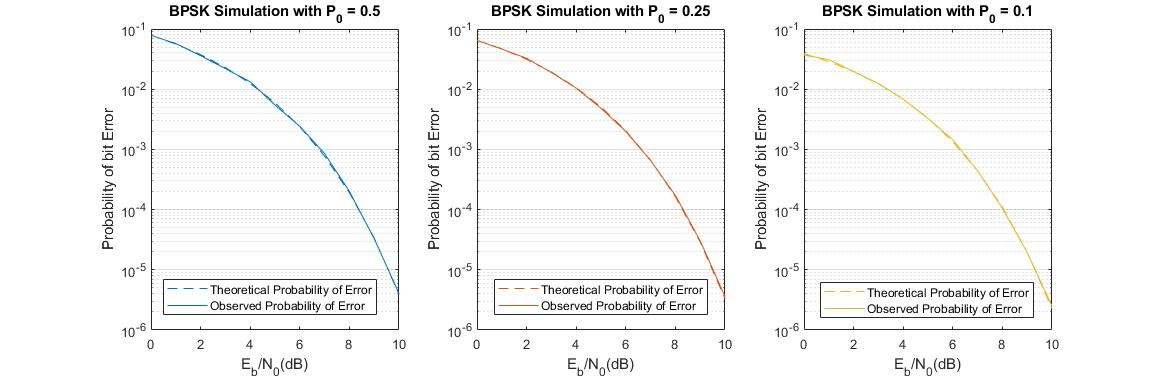
\includegraphics[width=\textwidth]{BPSKProbabilityBitError.jpg}
\item {\it Prompt: } Compare the theoretical and simulated results. Comment on the accuracy of the simiulation and the amount of time it tool to run the simulation. Comment on the importance of the theoretical models (where it is possible to obtain them). \\[0.05in]
			{\it Response: } In the plots above, we see that the simulated results closely resemble the theoretical results. It was helpful to have a mathematical description of what to expect because it helped to thoroughly test the code at a system level and identify errors. These results were also repeatable, although I did require that each simulation achieve at least 100 errors before terminating which helped manage the variability in the results. Fortunately, 100 errors wasn't overly taxing from a compute power perspective, especially with lower SNR values. With SNR values of $0$ to $6$, the simulation would run in several seconds, however when we started simulating values in the range of $9$ or $10$ the simulations could take as much as a minute to run. I can see how simulating performance with SNR values of 20 or more could require more time.
\item {\it Prompt: } Plot the probability of error for $P_0 = 0.1, P_0 = 0.25$ and $P_0 = 0.5$ on the same axes. Compare them and comment. \\[0.05in]
			{\it Response: } Observe the the probability of error for the three scenarios given below: \\
\begin{center}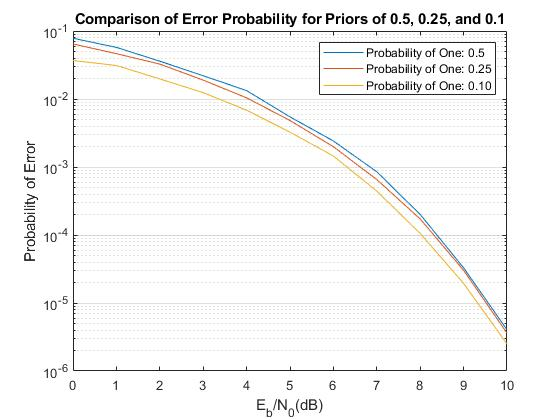
\includegraphics[width=\textwidth]{BPSKProbabilityBitErrorAll.jpg}\end{center}
and how the probability of error seems to decrease as the prior probability becomes more certain. Better performance with a more polarized probability is expected because the system's behavior is more predictable. By modifying the likelihood function to account for the difference in probability distributions we effectively encorporate more information into our system.  
\end{enumerate}
\problemsep
\pagebreak \begin{center} \vspace{-0.2in} \underline{8-PSK Simulation} \end{center}
\begin{itemize}
	\item {\it Prompt: }Write a program that will simulate an 8-PSK communication system with equal prior bit probabilities. Use a signal constellation in which the pointsnumbered in Gray code order. Make your program so that you can estimate botht eh symbol error probability and the bit error probability. Decide on an appropriate value of $N$. \\[0.05in]
				{\it Response: } This was accomplished in tandom with the BPSK code given in the previous section. The only change was to use an $N$ of 10000 because there were more errors in this simulation.
	\item {\it Prompt: } Prepare data from which to plot the bound on the probability of symbol error $P_s$ using (1.26) and the probability of bit error $P_b$ using (1.28). \\[0.05in]
				{\it Response: } This was accomplished as part of the PerformanceMetric class given above.
	\item {\it Prompt: }Plot the simulated probability of symbol error and bit error on the same axes as the bounds on the probabilities of error.\\[0.05in]
				{\it Response: } A plot containing each of these elements is given below.
\begin{center}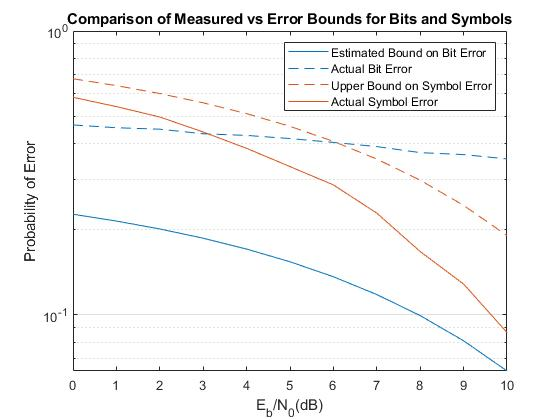
\includegraphics[width=\textwidth]{8PSKProbabilityError.jpg}\end{center}
	\item {\it Prompt: } Compare the theoretical and simulated results. Comment on the accuracy of the bound compared to the simulation and the amount of time it took to run the simulation. \\[0.05in]
				{\it Response: } The theoretical results did act as an upper bound, although the accuracy of the bounds is rather poor.  If feels like if these bounds are the only estimate available, then there is a good chance I would end up overdesigning a system because of their lack of accuracy, especially when estimating the error bounds for the probability of bit error. In regards to the simulation compute time, this particular simulation was run with a minimum error count of 10000 and ran relatively quick, requiring 5 - 10 seconds to complete. 
\end{itemize}

\problemsep
\pagebreak \begin{center} \vspace{-0.2in} \underline{Coded BPSK Simulation} \end{center}
\begin{enumerate}
	\item {\it Prompt: } Write a program that will simulate performance of the $(7,4)$ Hamming code over a BSC channel with channel crossover probability $p=Q(\sqrt{2E_b/N_0})$ and plot the probability of error as a function of $E_b/N_0$ in dB. On the same plot, plot the theoretical probability of error for uncoded BPSK transmission. Identify what the coding gain is for a probability of error $P_b = 10^{-5}$.\\[0.05in]
				{\it Response: } Per the suggestions given in the problem description, I put together a BinarySymmetricChannel and HammingCode class that are shown below:
\lstinputlisting{src/BinarySymmetricChannel.h}
\lstinputlisting{src/HammingCode74.h}
\lstinputlisting{src/HammingCode1511.h}
and used the resulting probability of errors to generate the plot given below:
\begin{center}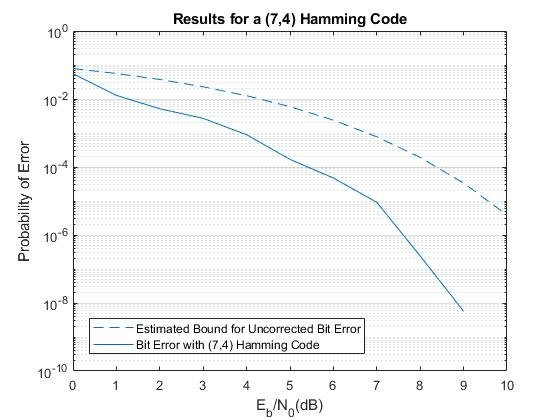
\includegraphics[width=\textwidth]{BPSKProbabilityError74Hamming.jpg}\end{center}
Note the improved performance between the two which demonstrates a coding gain of about 2.8 dB.
	\item {\it Prompt: } Repeat this for a (15,11) Hamming code. (See page 112 and Equations (3.6) and (3.4).) \\[0.05in]
			  {\it Response: } The performance of the (15,11) code was much better than the uncoded version although not quite as robust as its (7,4) counterpart with a 2.6 dB coding gain (approximately) as shown below:
\begin{center}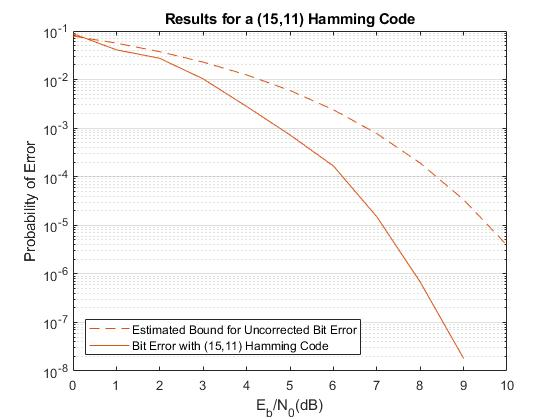
\includegraphics[width=\textwidth]{BPSKProbabilityError1511Hamming.jpg}\end{center}
\end{enumerate}

\end{document}
